\documentclass{article}
\usepackage{amsmath,amsfonts,amssymb,amscd,amsthm,xspace}
\usepackage[pdftex]{graphicx}     
\usepackage[T1]{fontenc}
\usepackage{titling}
\usepackage{enumitem}
\usepackage{float}
\usepackage{hyperref}

\usepackage{geometry}
\geometry{legalpaper, margin=1.5in}

\newcommand\tab[1][1cm]{\hspace*{#1}}

\title{ASSIGNMENT 2}
\date{Due date: 08:30, 19th October 2017}
\author{By Silas Jeppe Christensen}

\begin{document}
	\maketitle
	\subparagraph{}
	\begin{enumerate}
		\item Which language does the regular expression $\epsilon$ represent?\\
		It represent the language $\{\epsilon\}$
		\item Which language does the regular expression $\emptyset$ represent?\\
		It represent the the empty language $\{\} = \emptyset$ 
		\item Which language does the regular expression $a$ represent?\\
		It represent the the language \{a\}, respectively, where $a$ is an element of $\Sigma$. 
		\item Is it always true that $R + \epsilon$, where $R$ is a regular expression, represents the same language as $R$? If yes, explain. If not, give a counterexample\\
		Yes, becasue the resulting "new language" created by Union; $R \cup \epsilon$ still contains the same strings as in the previous "$R$".\\
		\item  For each of the following languages L, state whether or not L is regular. Prove your answer: 
		\begin{enumerate}[label=(\alph*)]
			\item \{$a^{i}b^{j} : i,j$ and $i + j = 5$\}\\
			\begin{figure}[H]
				\centering
				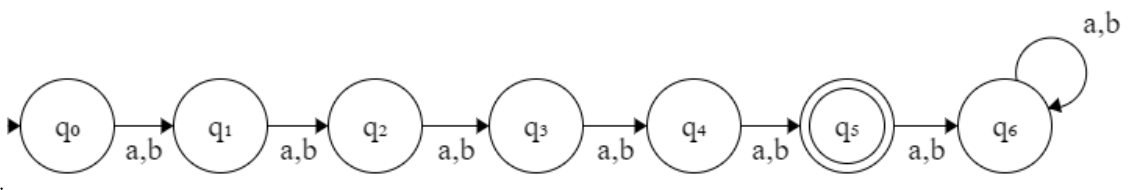
\includegraphics[width=0.7\linewidth]{5a}
				\caption{}
				\label{fig:5a}
			\end{figure}
			This exercise is a regular language, because if it's possible to draw a Finite Automata, the language is recognizable. Which means that the language is a regular language.
			\item \{$a^{i}b^{j} : i,j$ and $i - j = 5$\}\\
			This exercise will be proven by Pumping Lemma.\\
			By $a^ib^j \rightarrow i-j = 5 \leftrightarrow$ \\
			By assuming $k + l = i$, we can use xyz like this:\\
			$a^ka^lb^j$ where:\\
			$x = a^k$\\
			$y = a^l$\\
			$z = b^j$\\
			Then by pumping y 3 times: "$3 \times y = 3y$"\\
			Now we can tell that $k+l-j + 2l \neq k + l -j$.\\
			This exercise does not contain a regular language.
			\item \{$a^{i}b^{j} : i,j$ and $|i - j| \cong 0$ mod $5$\} I.e count a's (mod 5), then count b's (mod 5) and accepts iff the two counts are equal
			By assumtion:\\
			$i = 5 * k + l$\\
			$j = 5 * m + l$\\
			$i - l \% 5 = 0 \land j - l \% 5 = 0$\\
			$|i - j| \% 5 = 0$ for every $0\leq l \le 5$ \\ 
			$a^ta^vb^j \rightarrow t + v = i$\\
			$x = a^t$\\
			$y = a^v$\\
			$z = b^j$\\
			Then by pumping y 3 times ($3 \times y = 3y$), we end out with the function looking like:\\
			$(t + v - j) \% 5 = 0 \neq (t + 3v - j) \% 5 = 0$. \\
			By using pumping lemma, this exercise does not contain a regular language. For some expamples this will stille end as a regular language, but will fail most of the time.
			\item \{$w \in \{ Y,N \}^{\star}$ $w$ contains at least two Y's and at most two N's \}
			Regular like exercise 5a, since its possible to make a FA for this language.\\~\\
			\textbf{PICTURE HERE!!}\\~\\
			\item \{$w \in \{ a,b \}^{\star}$ $w$ contains exactly two more b's than a's\}\\
			L is a infinite language and if we assume that L is regular, we'll try to apply the pumping lemma. \\
			We'll end up with: $w = a^mb^{m+2}$. Then we can write down the xyz:\\
			xyz = $a^ka^lb^{m+2}$ where $k + l = m$ and:\\
			$x = a^k$\\
			$y = a^l$\\
			$z = b^{m+2}$\\
			Now, by using the pumping lemma, we can tell if the language is regular or not. Because pumping lemma states that $xy^iz \in L$, even if $i=0$. This leaves us with $xz \in L$. But for this language, that's is not the case, since $xz = a^{k-l}b^{m+2} \notin L$, $k + l = m$ and $k - l \neq m$. In this case L is not regular, since $xz \notin L$.
			\item \{$w \in \{ a,b \}^{\star}$ the number of occurrences of the substring $ab$ is equal to the number of occurrences of the substring $ba$.\}
			\item \{$w \in \{(,)\}^{\star}$  the parentheses are balances\}
			\item \{$ww^R \in \{a,b\}^\star$\}
		\end{enumerate}
		\item Can you use the Pumping Lemma for regular languages to show that a language is regular? If yes, explain why. If no, explain why not. \\~\\
		Yes. This is from the Michel Sipser book: \textit{"Our technique for proving nonregularity stems from a theorem about regular
		languages, traditionally called the pumping lemma. This theorem states that all
		regular languages have a special property. If we can show that a language does
		not have this property, we are guaranteed that it is not regular."}
		\item Let $\Sigma = \{a,b\}$. Consider the following grammars.
		 \begin{enumerate}[label=(\alph*)]
		 	\item $S \rightarrow aS|Sb|\epsilon$
		 	\item $S \rightarrow aSa|bSb|a|b$
		 	\item $S \rightarrow aS|bS|\epsilon$
		 	\item $S \rightarrow aS|aSbS|\epsilon$
		 \end{enumerate}
	For each language defined by the grammars, do the following:
		\begin{enumerate}[label=(\alph*)]
			\item  List five strings that are in L.
			\item  List five strings that are not in L.
			\item Describe L concisely. You can use regular expressions, set theoretic expressions, etc.
			\item  Indicate whether or not L is regular. Prove your answer.
		\end{enumerate}
		\item  Consider the following grammar $G : S \rightarrow 0S1|SS|10$.\\
		Show a parse tree produced by G for each of the following strings:
		\begin{enumerate}[label=(\alph*)]
			\item 010110	
			\begin{figure}[H]
				\centering
				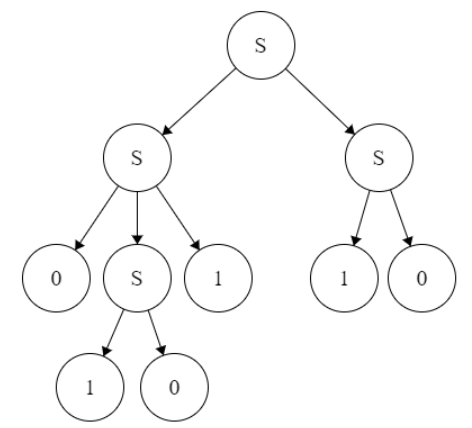
\includegraphics[width=0.7\linewidth]{8a}
				\caption{}
				\label{fig:8a}
			\end{figure}
			\item 00101101
			\begin{figure}[H]
				\centering
				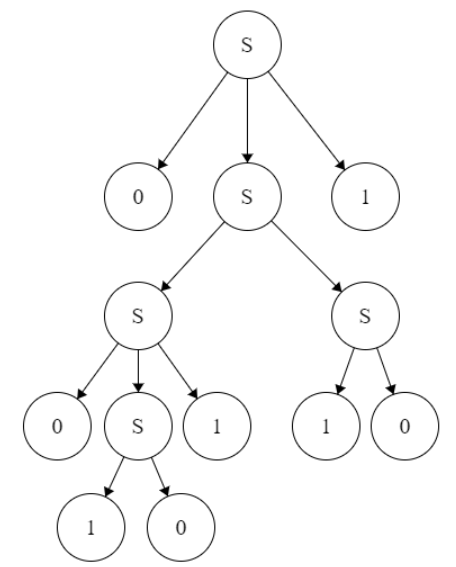
\includegraphics[width=0.7\linewidth]{8b}
				\caption{}
				\label{fig:8b}
			\end{figure}
		\end{enumerate}
	\end{enumerate}
\end{document}